\section{Experiments and Results}
\label{sec:results}

All our experiments have been completed with the inexpensive consumer
quadcopter called Parrot's AR Drone 2.0. We have used the ROS based
ARDrone Autonomy Driver to communicate with the drone. For the
purposes of establishing the ground truth, pictures were taken with a
5 mega pixel camera.

We have implemented our algorithm in C++ using the OpenCV library
(OpenCV 2.4.9). Experiments were performed on a PC with Intel Core i7
processor(@3.4GHz) and 8GB RAM.  The source code to produce
interesting images from a video, and to generate the super-panorama,
as well as the data sets used in this paper will be made publicly
available.


\subsection{Establishing Correctness}

In our first experiment, we wanted to ensure that the selection of
images done was comprehensive.  We sent the drone to recce an outdoor
scene with no dead space. This experiment was conducted in an outdoor
environment. We note here that there were approximately 9000 images in
the raw video.  Autostitch was unable to cope when fed with this large
number. 

One way to produce some sort of mosaic was to simply reduce the amount
of data given to Autostitch.  Figure \ref{fig:uniformsampled_sac3}
shows uniformly time sampled images from complete video.  When these
uniformly sampled images are given to Autostitch or to Adobe
Photoshop, we find (Fig.~\ref{fig:results_sac3_timesmapled})  that the
results are not satisfactory.

Instead of feeding time-sampled images, we ran our saliency selection
algorithm on the video. Fig.~\ref{fig:selected_sac3} shows examples of
selected images. Many of the images are similar to the time sampled
version; however, the occasional differences are enough to make
Autostitch work. 

Using only $N=5$ images, the results are shown in
Fig.~\ref{fig:results_sac3_timesmapled}.


\begin{figure*}[htb!]
\centering
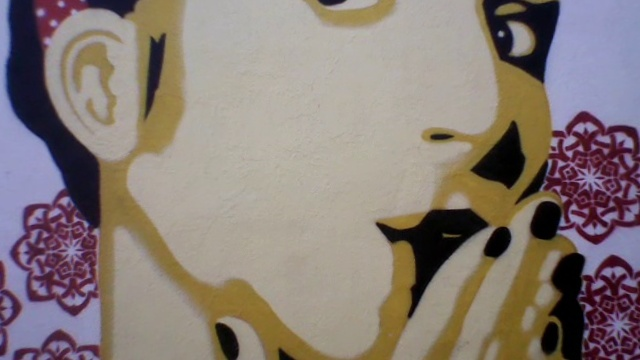
\includegraphics[width=0.19\linewidth]{figures/sac3/uniform_sampled/1.jpg}
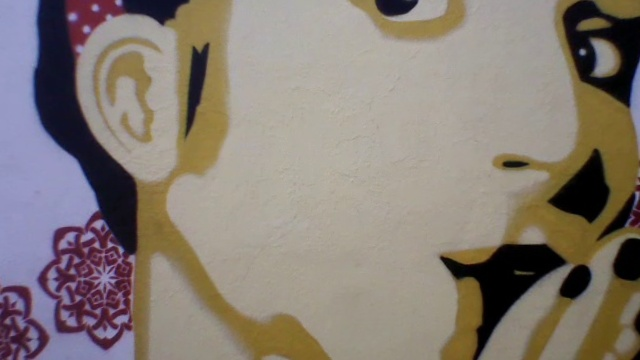
\includegraphics[width=0.19\linewidth]{figures/sac3/uniform_sampled/5.jpg}
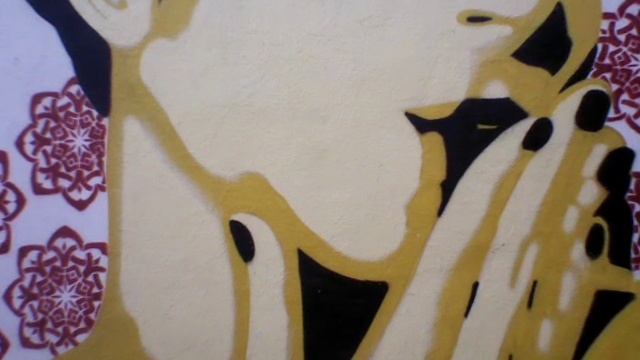
\includegraphics[width=0.19\linewidth]{figures/sac3/uniform_sampled/4.jpg}
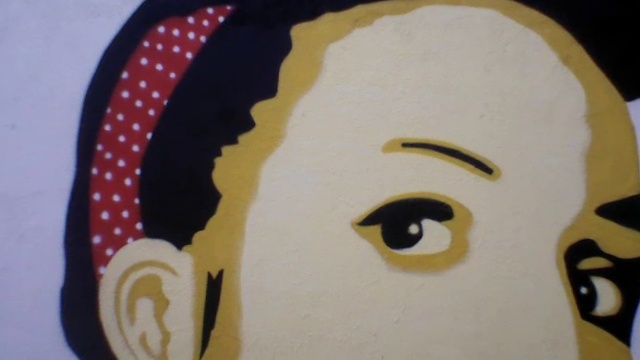
\includegraphics[width=0.19\linewidth]{figures/sac3/uniform_sampled/2.jpg}
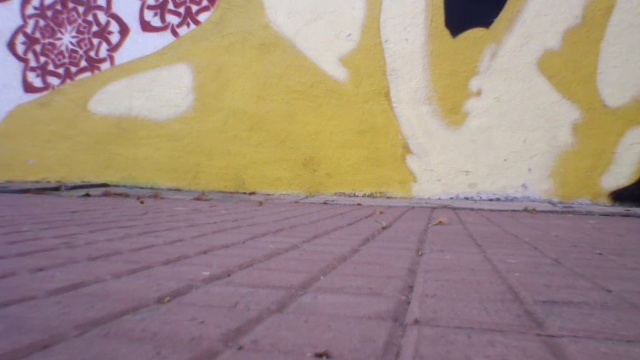
\includegraphics[width=0.19\linewidth]{figures/sac3/uniform_sampled/3.jpg}
\caption{Uniformly sampled images from an outdoor video expedition.}
\label{fig:uniformsampled_sac3}
\end{figure*}

\begin{figure*}[t!]
\centering
\begin{subfigure}[b]{0.4\textwidth}
\centering
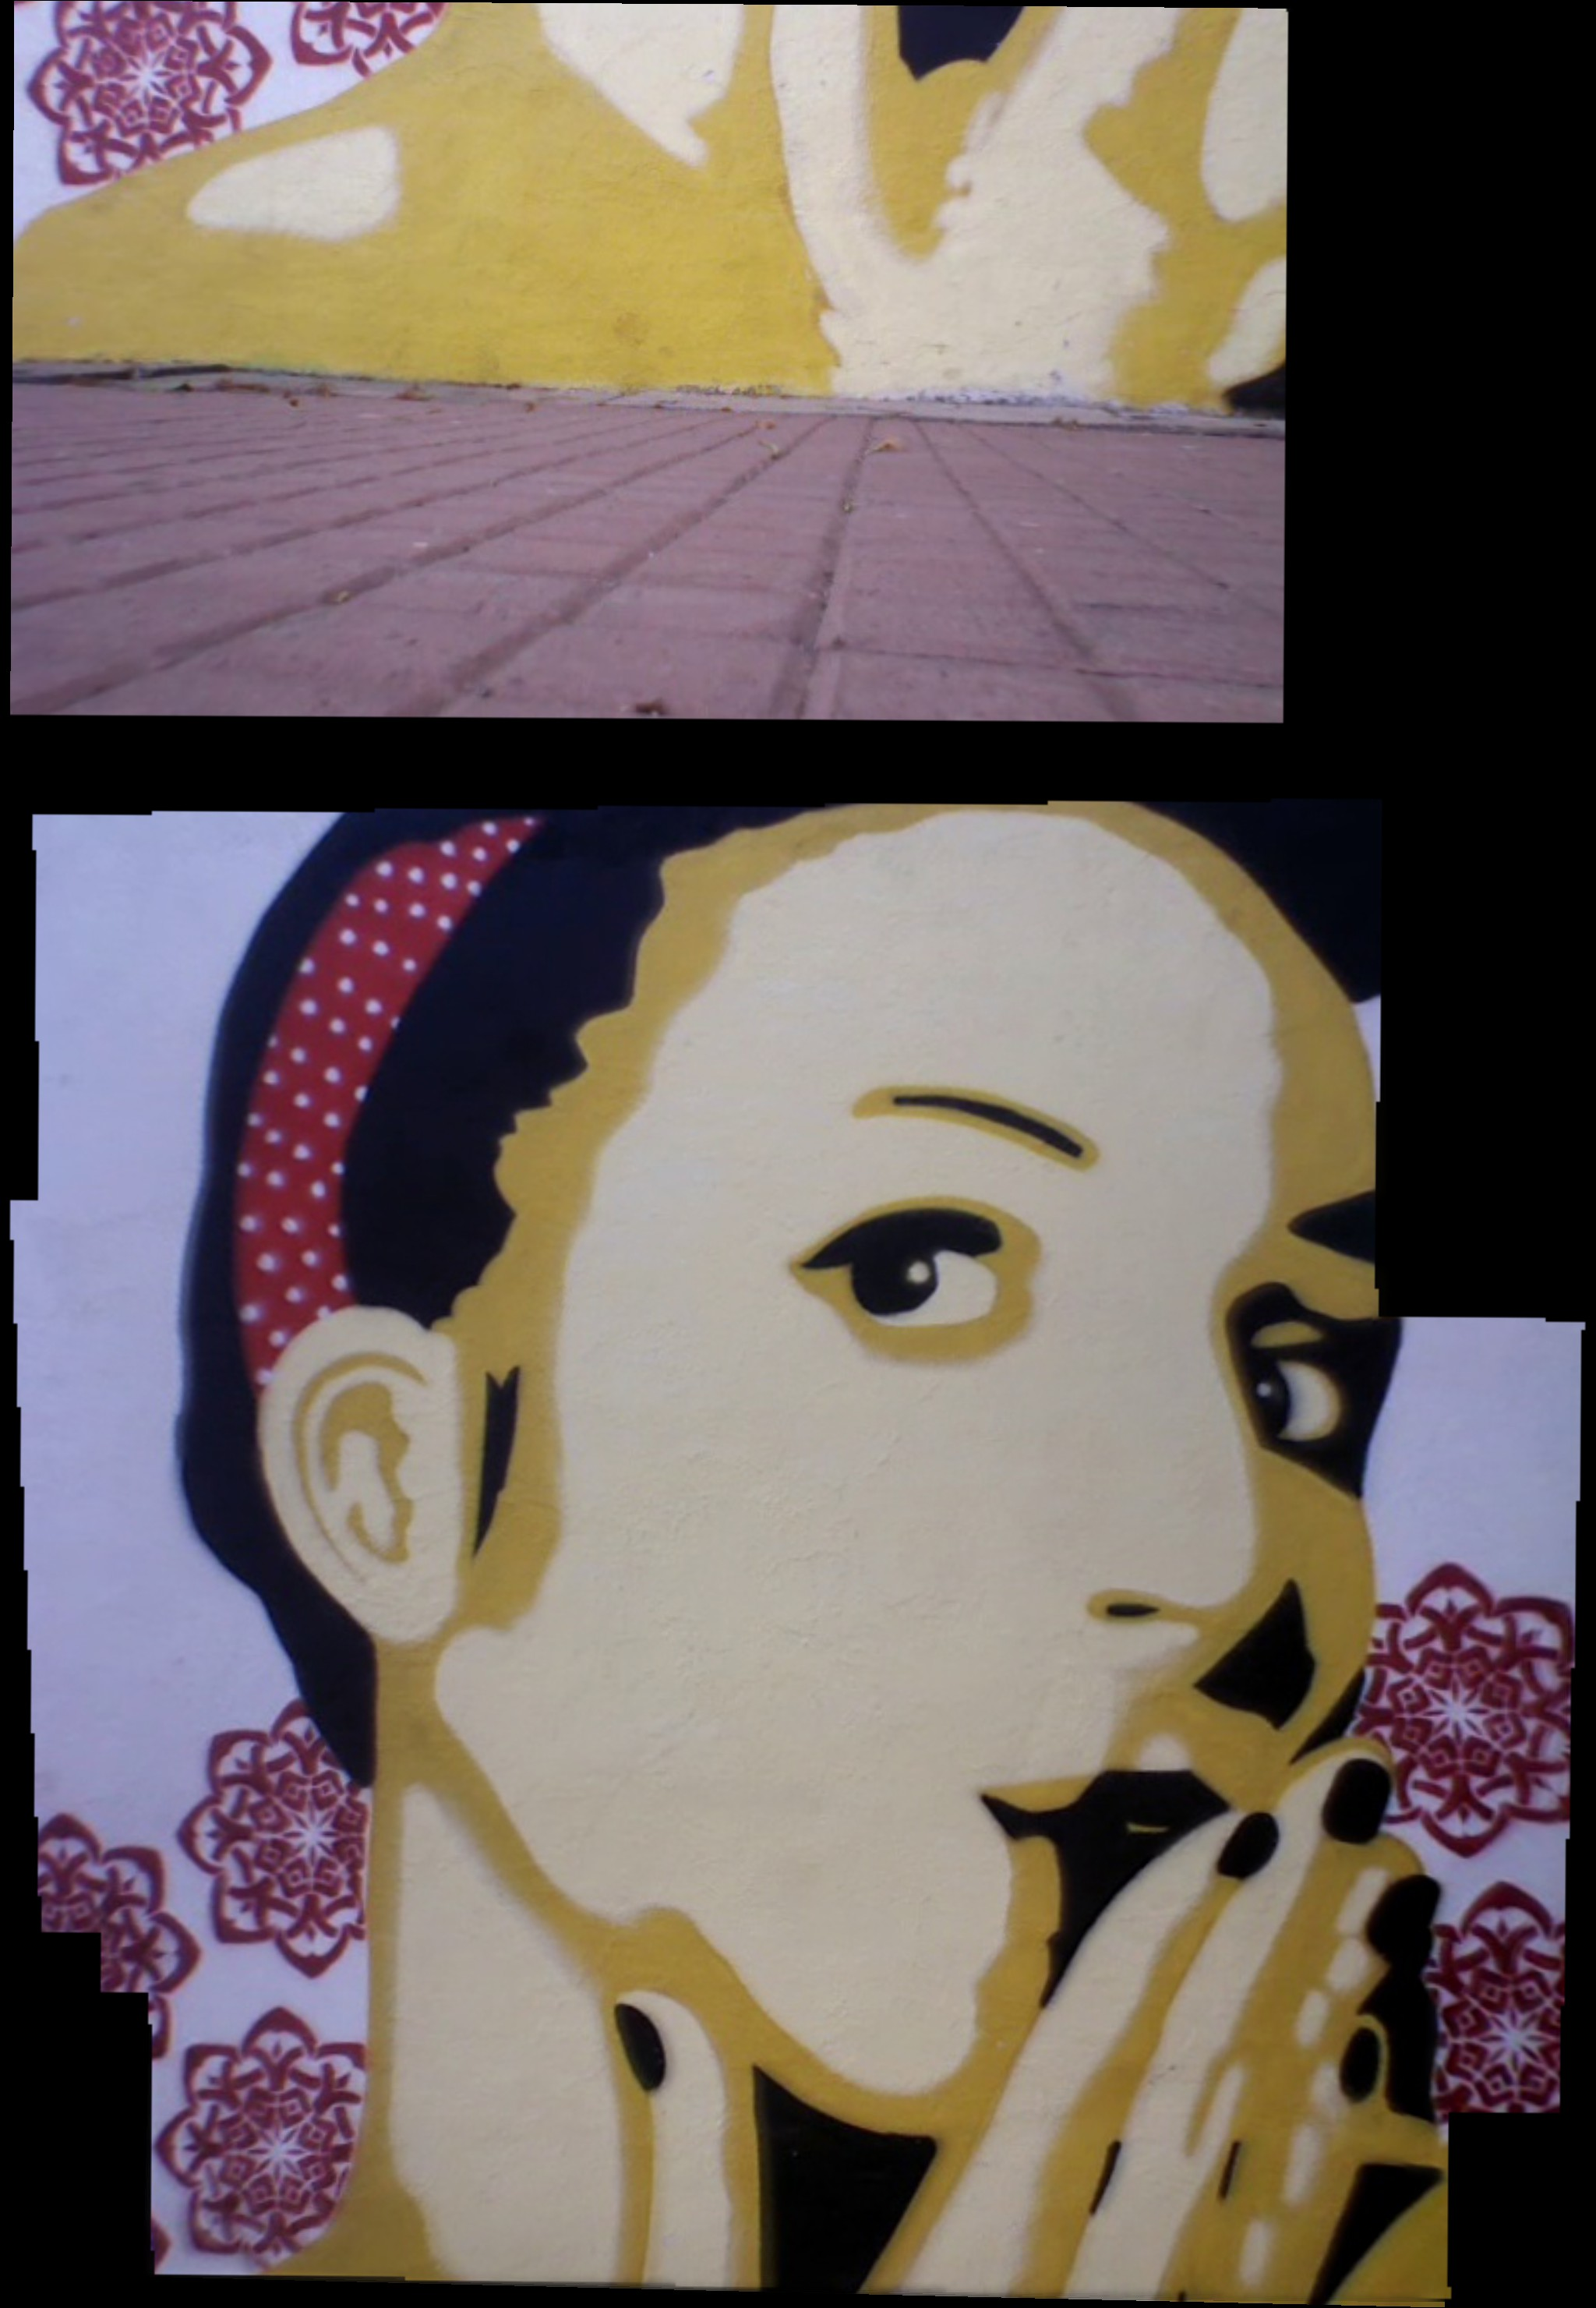
\includegraphics[width=\linewidth]{figures/sac3/uniform_sampled/autostitch.jpg}
\caption{Autostitch Result}
\end{subfigure}
\begin{subfigure}[b]{0.4\textwidth}
\centering
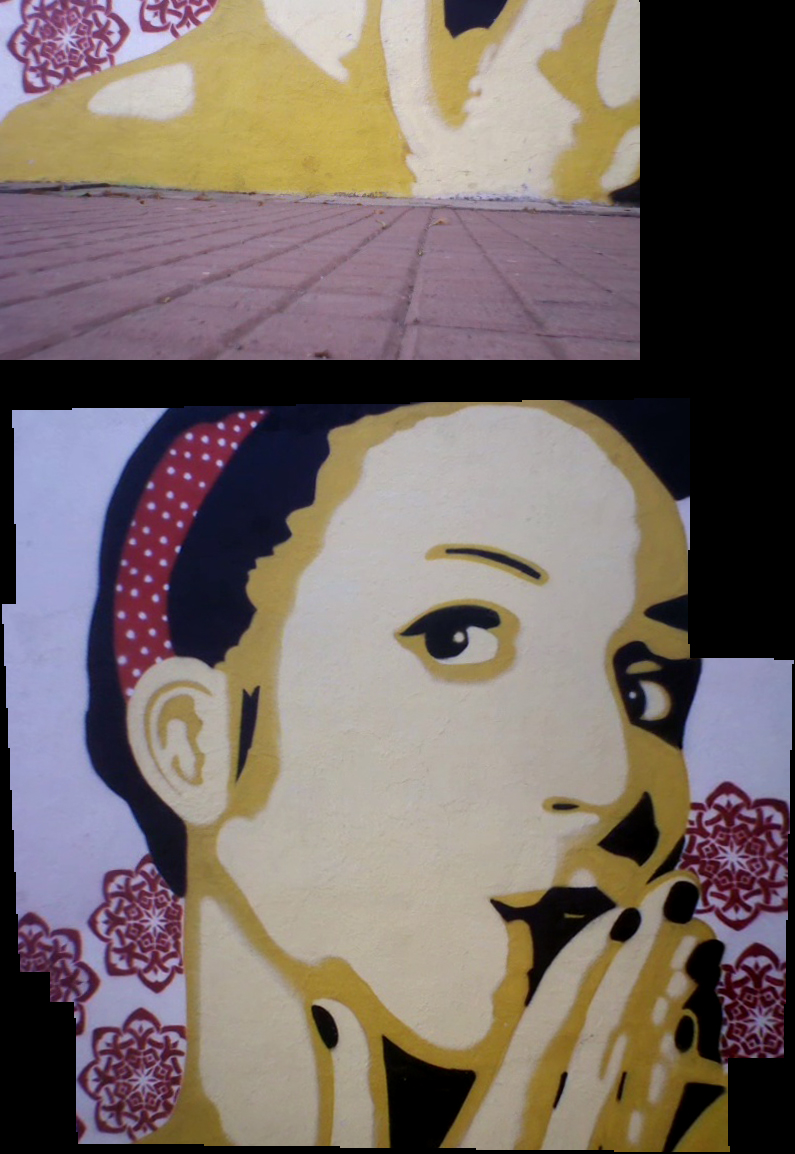
\includegraphics[width=\linewidth]{figures/sac3/uniform_sampled/photoshop.jpg}
\caption{Photoshop Result}
\end{subfigure}
\caption{Output of state of the art photo stitchers on uniformly time
  sampled images. As time sampled images do not guarantee 
  coverage of the scene, the panorama is broken. The top portions do
  not belong at the right place (see Fig.~\ref{fig:results_sac3})}
\label{fig:results_sac3_timesmapled}
\end{figure*}


\begin{figure*}[htb!]
\centering
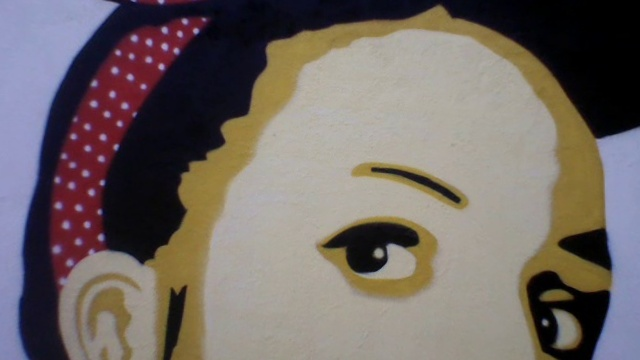
\includegraphics[width=0.19\linewidth]{figures/sac3/selected/1.jpg}
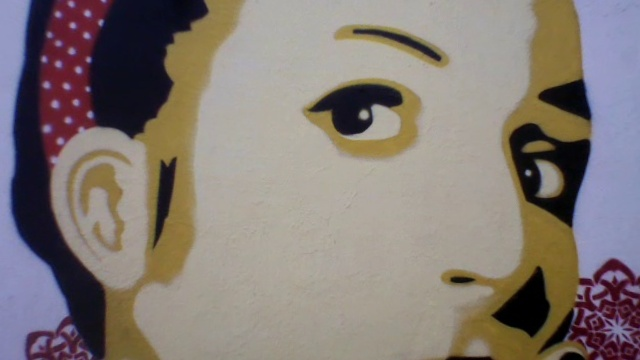
\includegraphics[width=0.19\linewidth]{figures/sac3/selected/5.jpg}
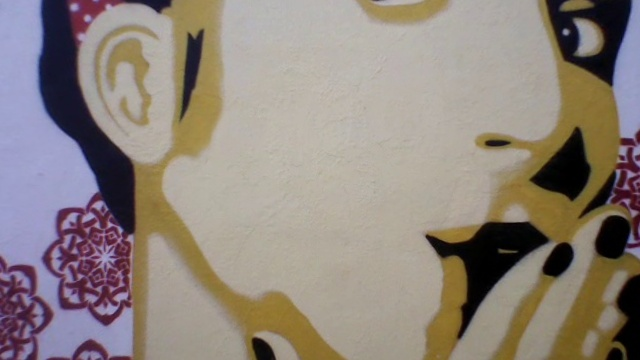
\includegraphics[width=0.19\linewidth]{figures/sac3/selected/4.jpg}
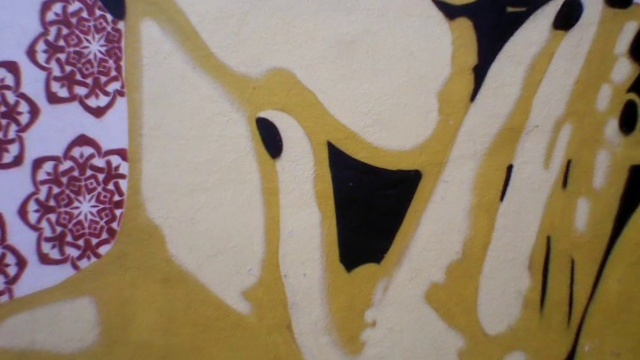
\includegraphics[width=0.19\linewidth]{figures/sac3/selected/2.jpg}
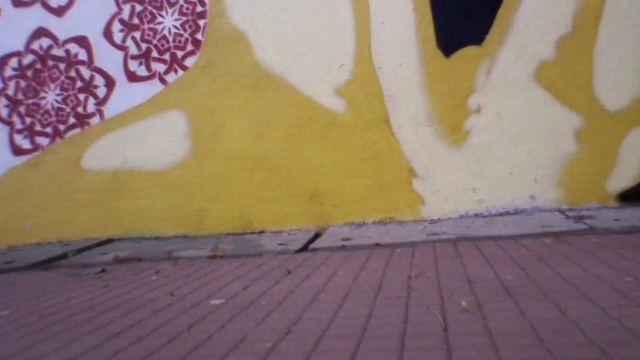
\includegraphics[width=0.19\linewidth]{figures/sac3/selected/3.jpg}
\caption{Salient image selection from the set of approximately 9000
  images using positional information.}
\label{fig:selected_sac3}
\end{figure*}


\begin{figure*}
\centering
\begin{subfigure}[b]{0.3\textwidth}
\centering
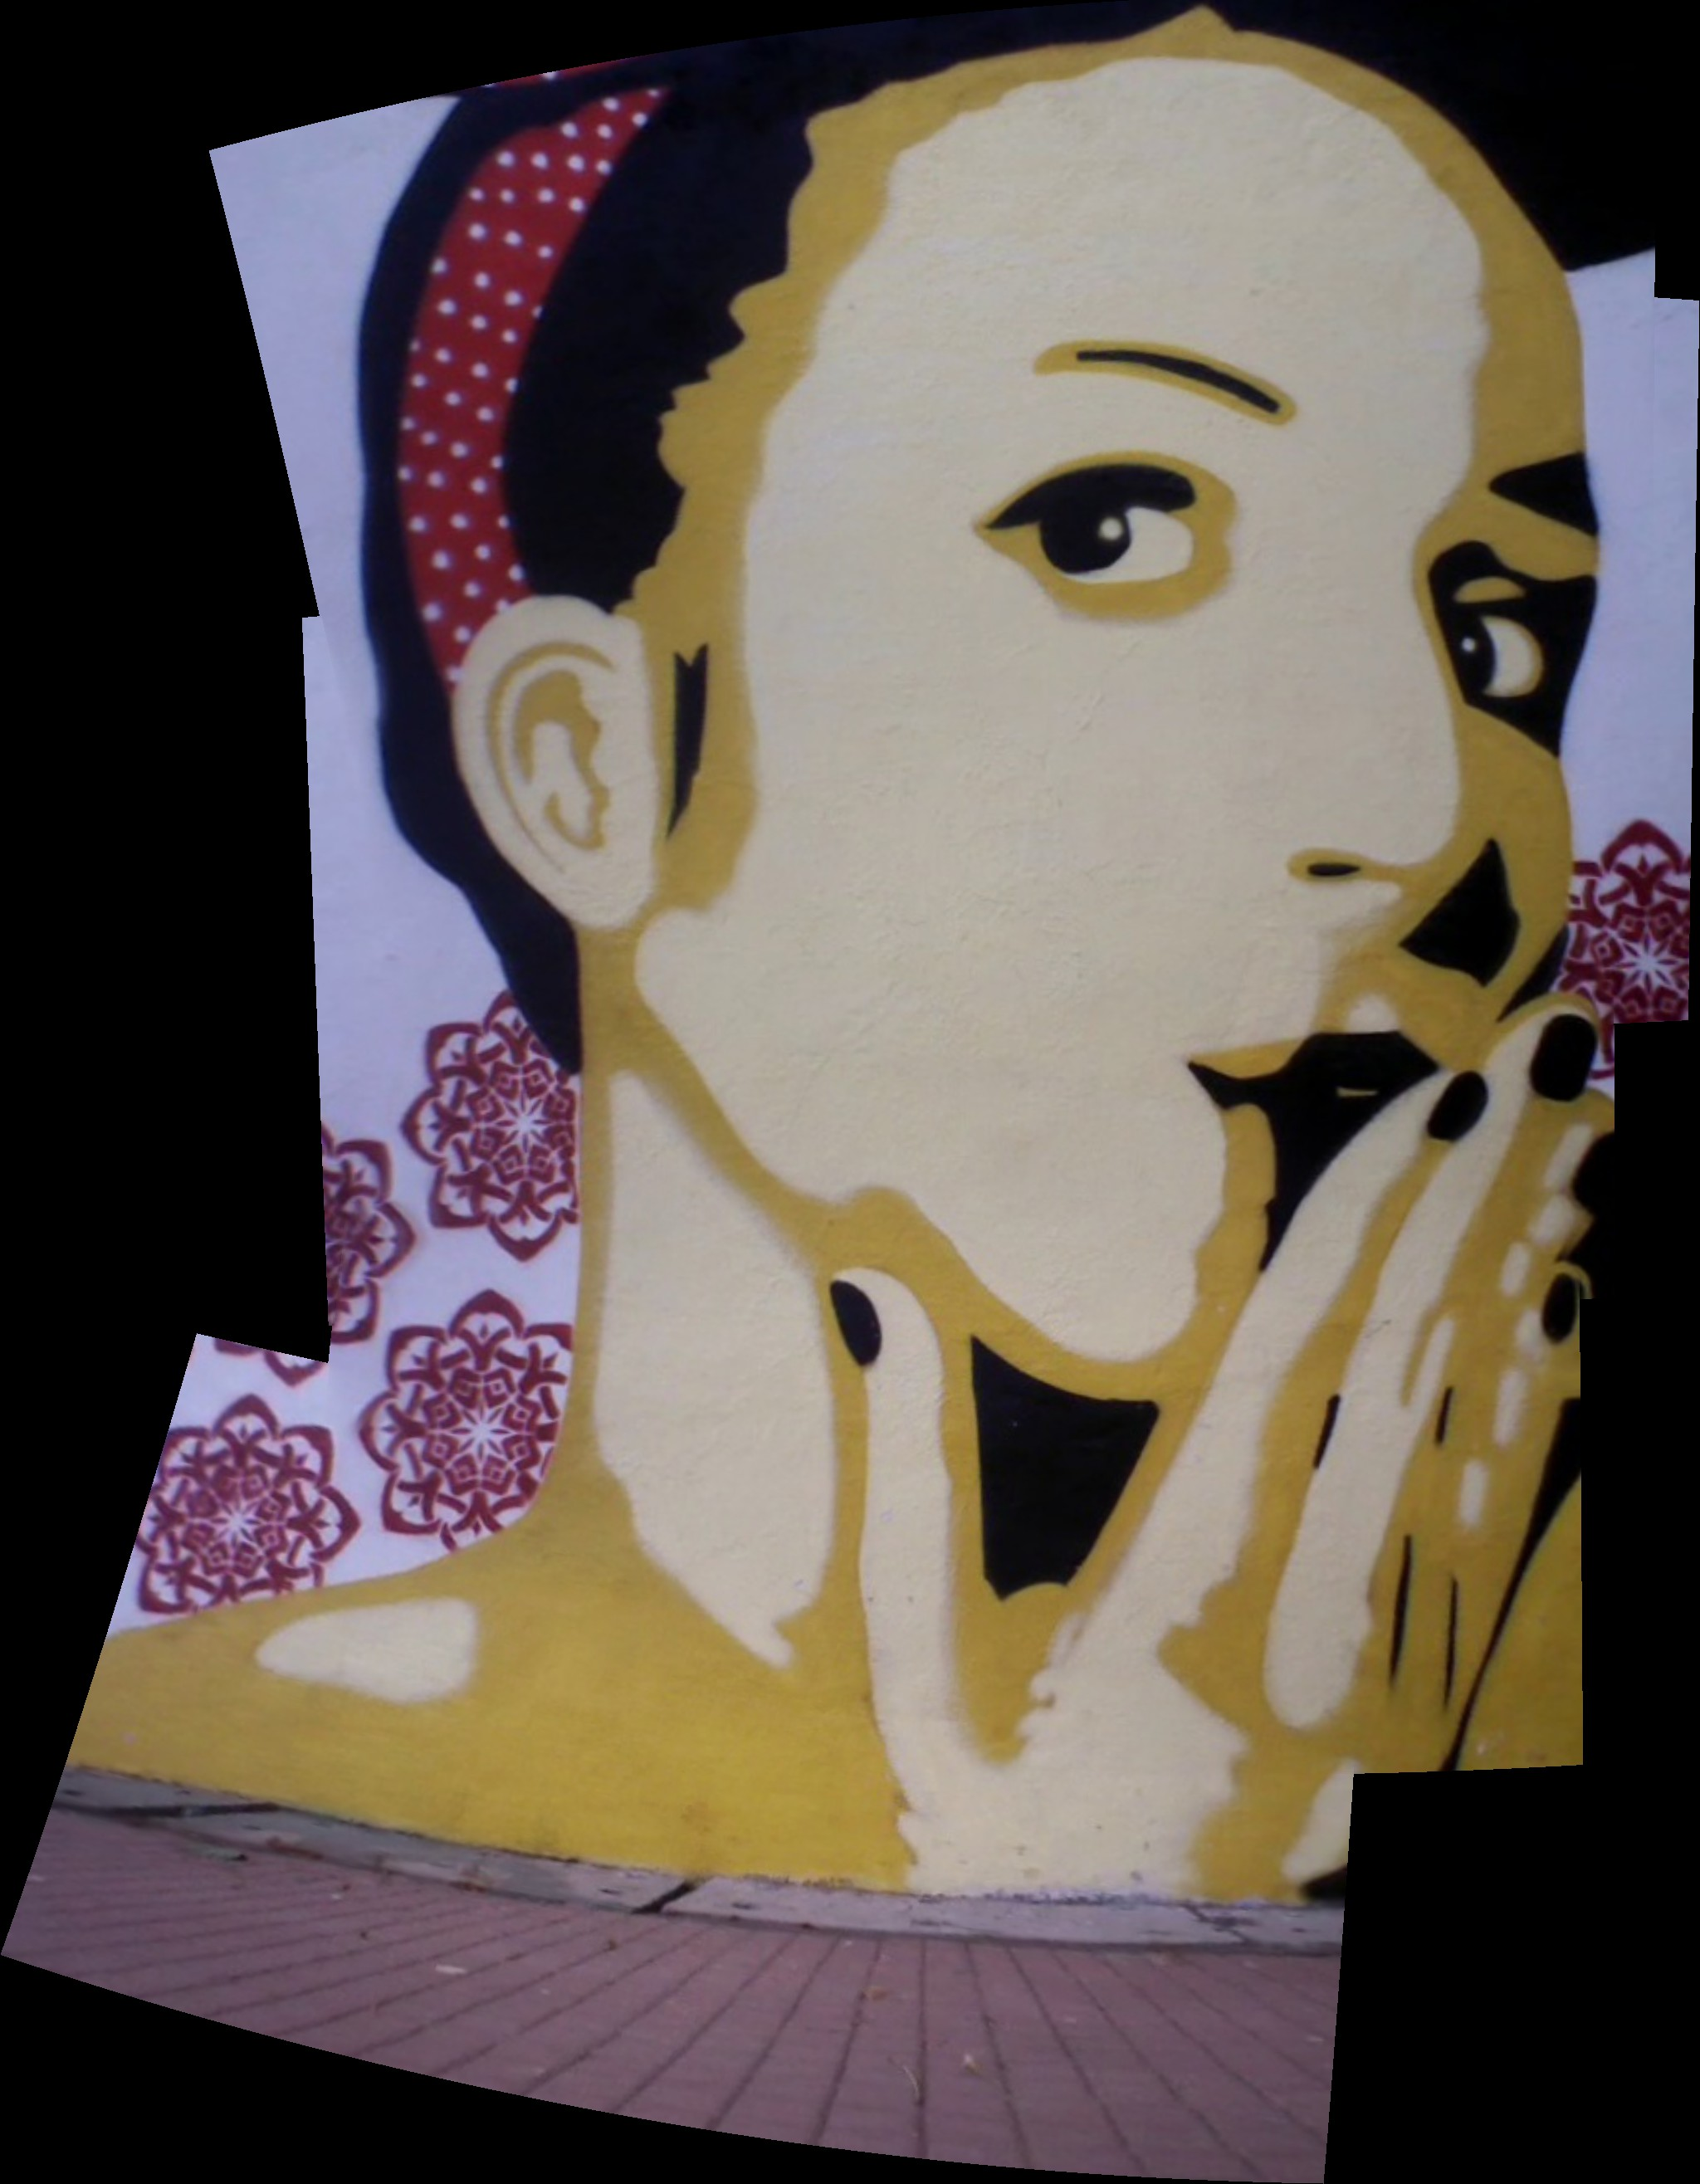
\includegraphics[width=\linewidth]{figures/sac3/autostitch.jpg}
\caption{Autostitch Result}
\end{subfigure}
\begin{subfigure}[b]{0.3\textwidth}
\centering
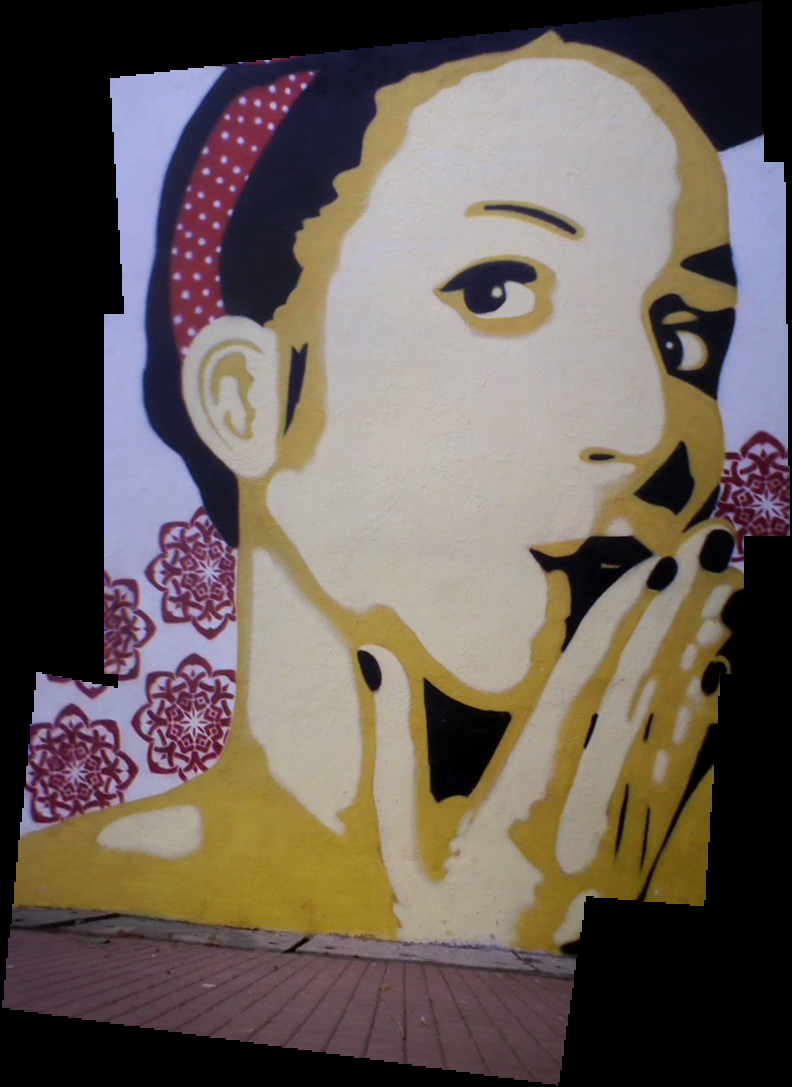
\includegraphics[width=\linewidth]{figures/sac3/photoshop.jpg}
\caption{Photoshop Result}
\end{subfigure}
\begin{subfigure}[b]{0.3\textwidth}
\centering
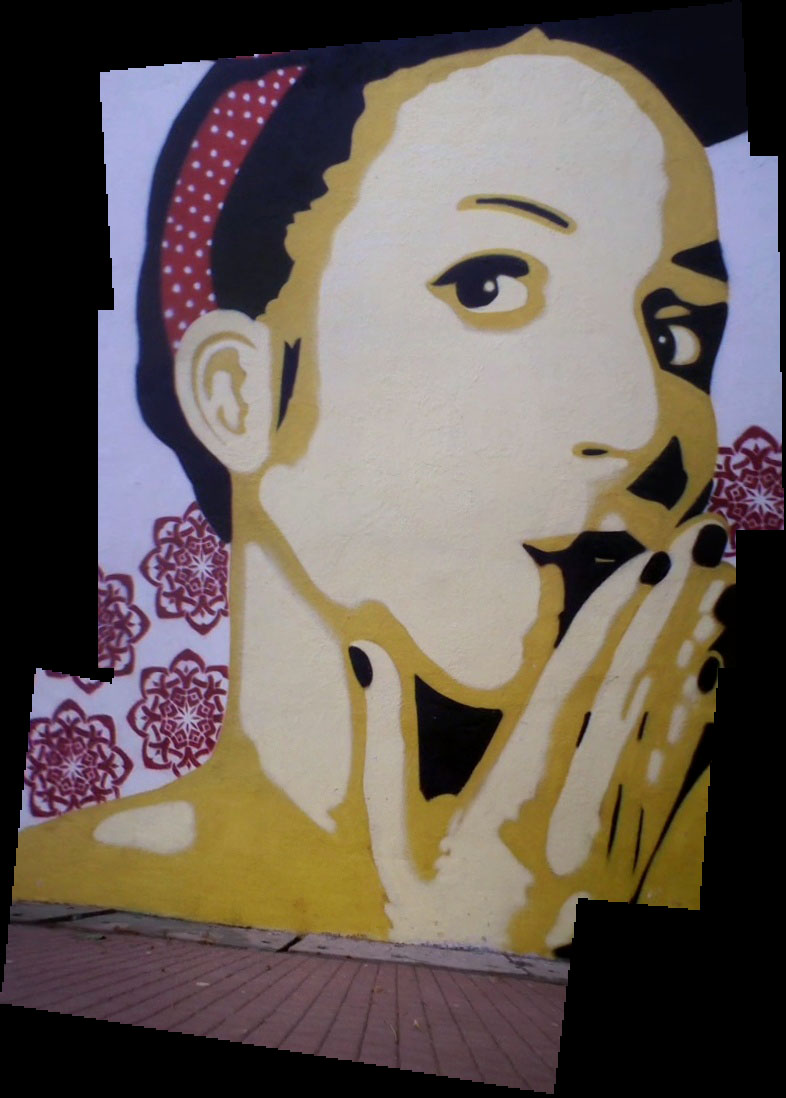
\includegraphics[width=\linewidth]{figures/sac3/our_result.jpg}
\caption{Our Result}
\end{subfigure}
\caption{When salient images are given to Autostich and Photoshop, a
  video can be used to create a panaromic mosaic provided there is no
  dead space. We also show the results from our stitching algorithm.}
\label{fig:results_sac3}
\end{figure*}

In summary, this experiment provides evidence to show that (a) our
saliency selection algorithm is reasonable and (b) our stitching
results are comparable to that of Autostitch for the kind of scenes
considered.

\subsection{Indoor Imagery with Dead Space} 

Our next selection of experiments were conducted in an indoor
environment with some natural light.  The input stream had about 4300
images. The selection algorithm pruned the video into N=4 images. A
sample of the selected images are seen in Fig.~\ref{fig:idc_selected}

\begin{figure}
\centering

\includegraphics[width=0.22\linewidth]{figures/idc_indoor/selected/1.jpg}

\includegraphics[width=0.22\linewidth]{figures/idc_indoor/selected/2.jpg}

\includegraphics[width=0.22\linewidth]{figures/idc_indoor/selected/3.jpg}

\includegraphics[width=0.22\linewidth]{figures/idc_indoor/selected/4.jpg}
\caption{Pruned images from a video of an indoor scene.}
\label{fig:idc_selected}
\end{figure}

There were two disconnected components in the resulting graph.
Autostitch was unable to produce any reasonable output as seen in
Figure~\ref{fig:idc_indoor_comparison}.  The ground truth can be seen
in Fig.~\ref{fig:idc_indoor_groundtruth}.  One can see a better
orthographic view of the posters in a composite manner.


\begin{figure}[p]
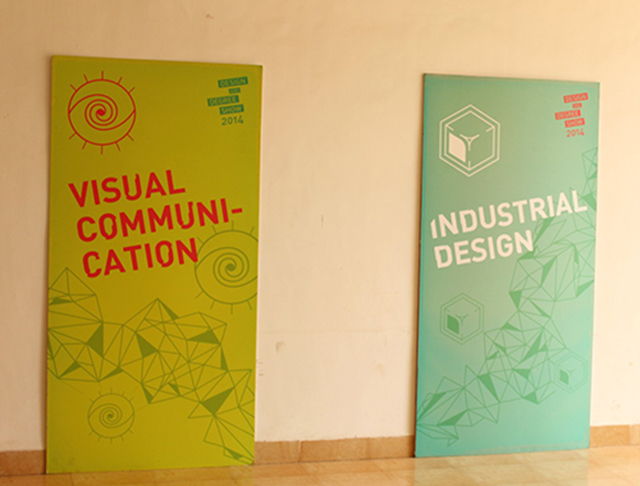
\includegraphics[width=\linewidth]{figures/idc_indoor/groundtruth.jpg}
\caption{Ground truth of the indoor scene.  There is a substantial gap
  in between the two posters, and this dead space confuses state of the
  art stitchers since they do not find features.}
\label{fig:idc_indoor_groundtruth}
\end{figure} 

Figure \ref{fig:idc_indoor_comparison} shows the comparison of outputs of state
of the art stitchers with output of our algorithm. 

\begin{figure*}
\begin{subfigure}[b]{0.3\textwidth}

\includegraphics[width=\linewidth]{figures/idc_indoor/autostitch.jpg}
\caption{Autostitch Result}
\end{subfigure}
\begin{subfigure}[b]{0.3\textwidth}

\includegraphics[width=\linewidth]{figures/idc_indoor/photoshop.jpg}
\caption{Photoshop Result}
\end{subfigure}
\begin{subfigure}[b]{0.3\textwidth}

\includegraphics[width=\linewidth]{figures/idc_indoor/our_result.jpg}
\caption{Our Result}
\end{subfigure}
\caption{Comparison of outputs of Autostich, Photoshop and our stitching
algorithm on an indoor scene. Only our
algorithm is able to show a complete super-panorama; state-of-the art
stitchers can produce only one mini-panorama.}
\label{fig:idc_indoor_comparison}
\end{figure*}

One can see a better orthographic view of the posters in a composite
manner. Autostitch was unable to produce any reasonable output as seen in
Figure \ref{fig:idc_indoor_comparison}.

\subsection{Outdoor Imagery with Dead Space}
Our next set of experiments were conducted in an outdoor environment. The  
input stream had about 12000 images. The selection algorithm pruned the video
into N=30 images. A sample of the selected images are seen in Figure
\ref{fig:green_red_selected}.

\begin{figure}
\centering
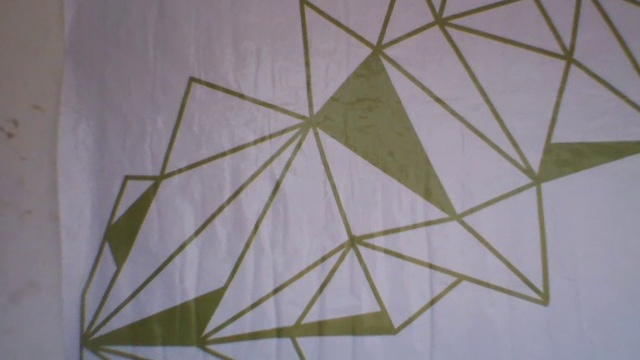
\includegraphics[width=0.19\linewidth]{figures/green_red/selected/1.jpg}
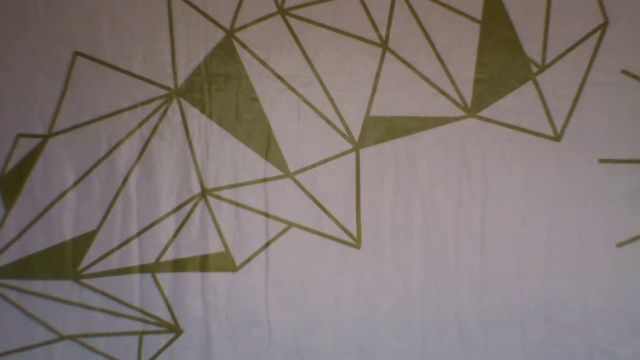
\includegraphics[width=0.19\linewidth]{figures/green_red/selected/2.jpg}
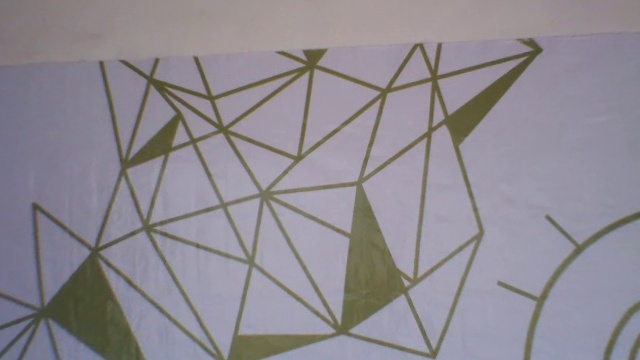
\includegraphics[width=0.19\linewidth]{figures/green_red/selected/3.jpg}
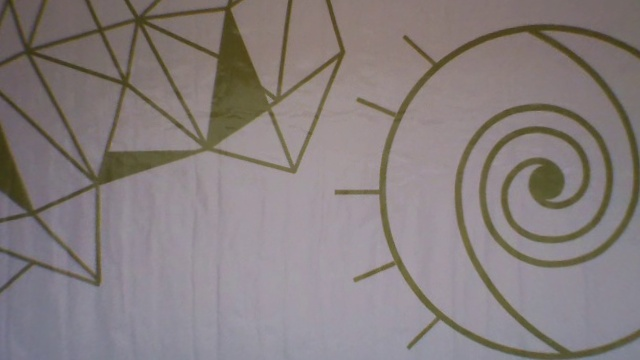
\includegraphics[width=0.19\linewidth]{figures/green_red/selected/4.jpg}
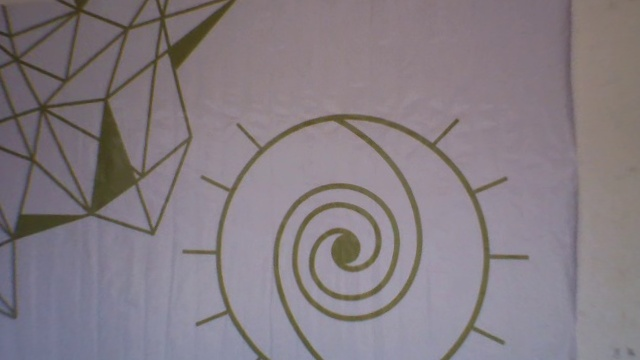
\includegraphics[width=0.19\linewidth]{figures/green_red/selected/5.jpg}
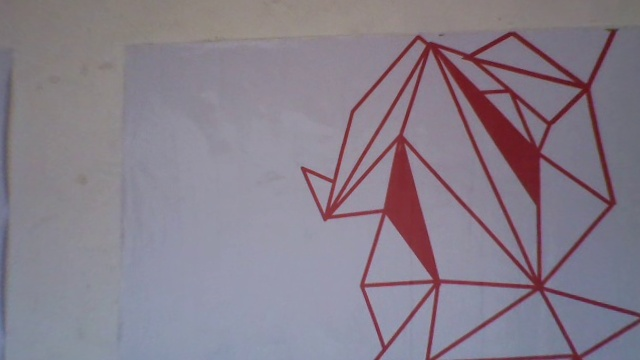
\includegraphics[width=0.19\linewidth]{figures/green_red/selected/6.jpg}
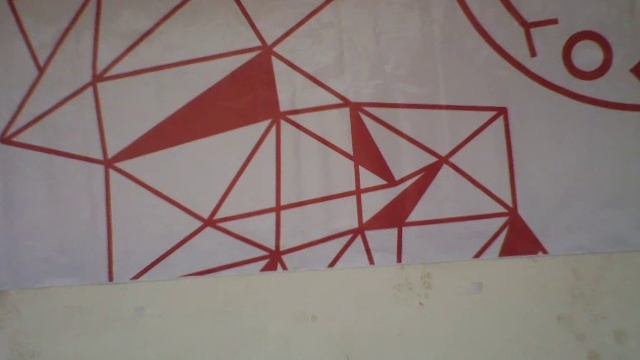
\includegraphics[width=0.19\linewidth]{figures/green_red/selected/7.jpg}
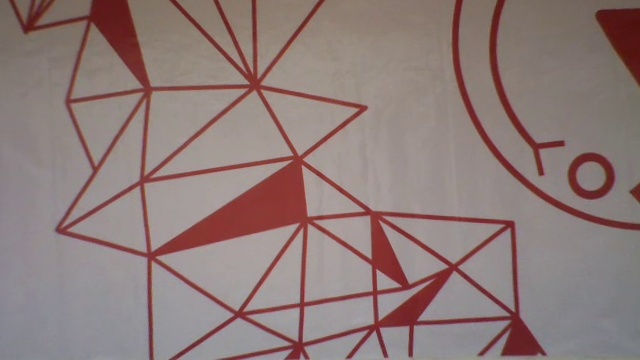
\includegraphics[width=0.19\linewidth]{figures/green_red/selected/8.jpg}

\includegraphics[width=0.19\linewidth]{figures/green_red/selected/9.jpg}
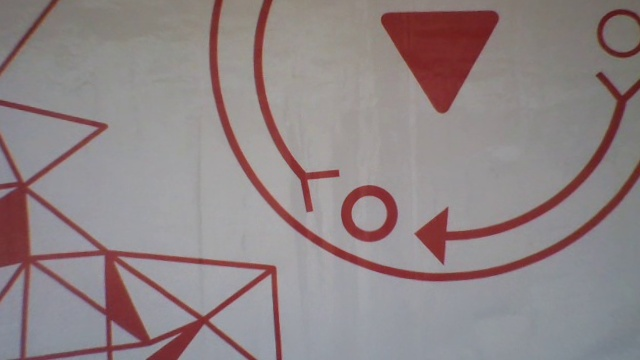
\includegraphics[width=0.19\linewidth]{figures/green_red/selected/10.jpg}
\caption{Sample selected images of outdoor scene by our algorithm.}
\label{fig:green_red_selected}
\end{figure}

The ground truth of outdoor scene can be seen in Figure
\ref{fig:green_red_groundtruth}.

\begin{figure}
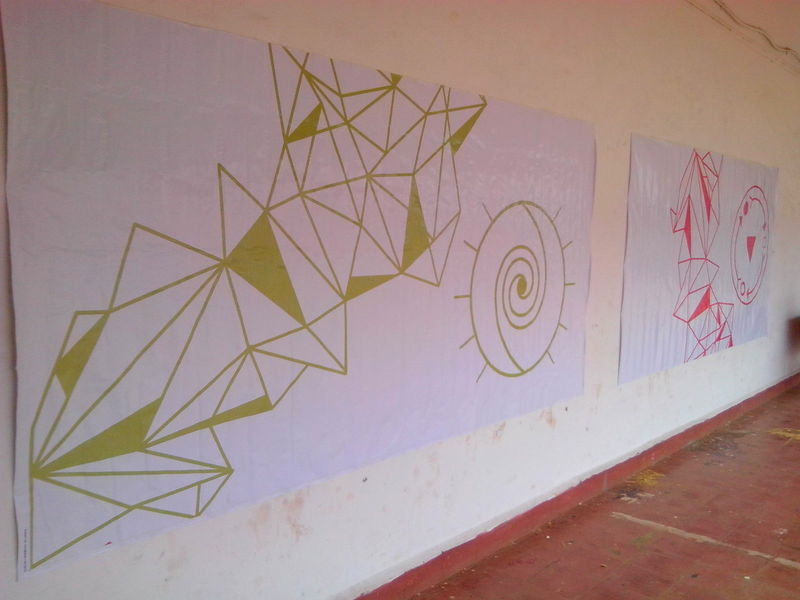
\includegraphics[width=\linewidth]{figures/green_red/groundtruth.jpg}
\caption{Ground truth of the outdoor scene captured by quadcopter. There is
visible gap in between two posters which will cause problems for state of the art
stitchers.}
\label{fig:green_red_groundtruth}
\end{figure}


\begin{figure*}
\begin{subfigure}[b]{0.3\textwidth}
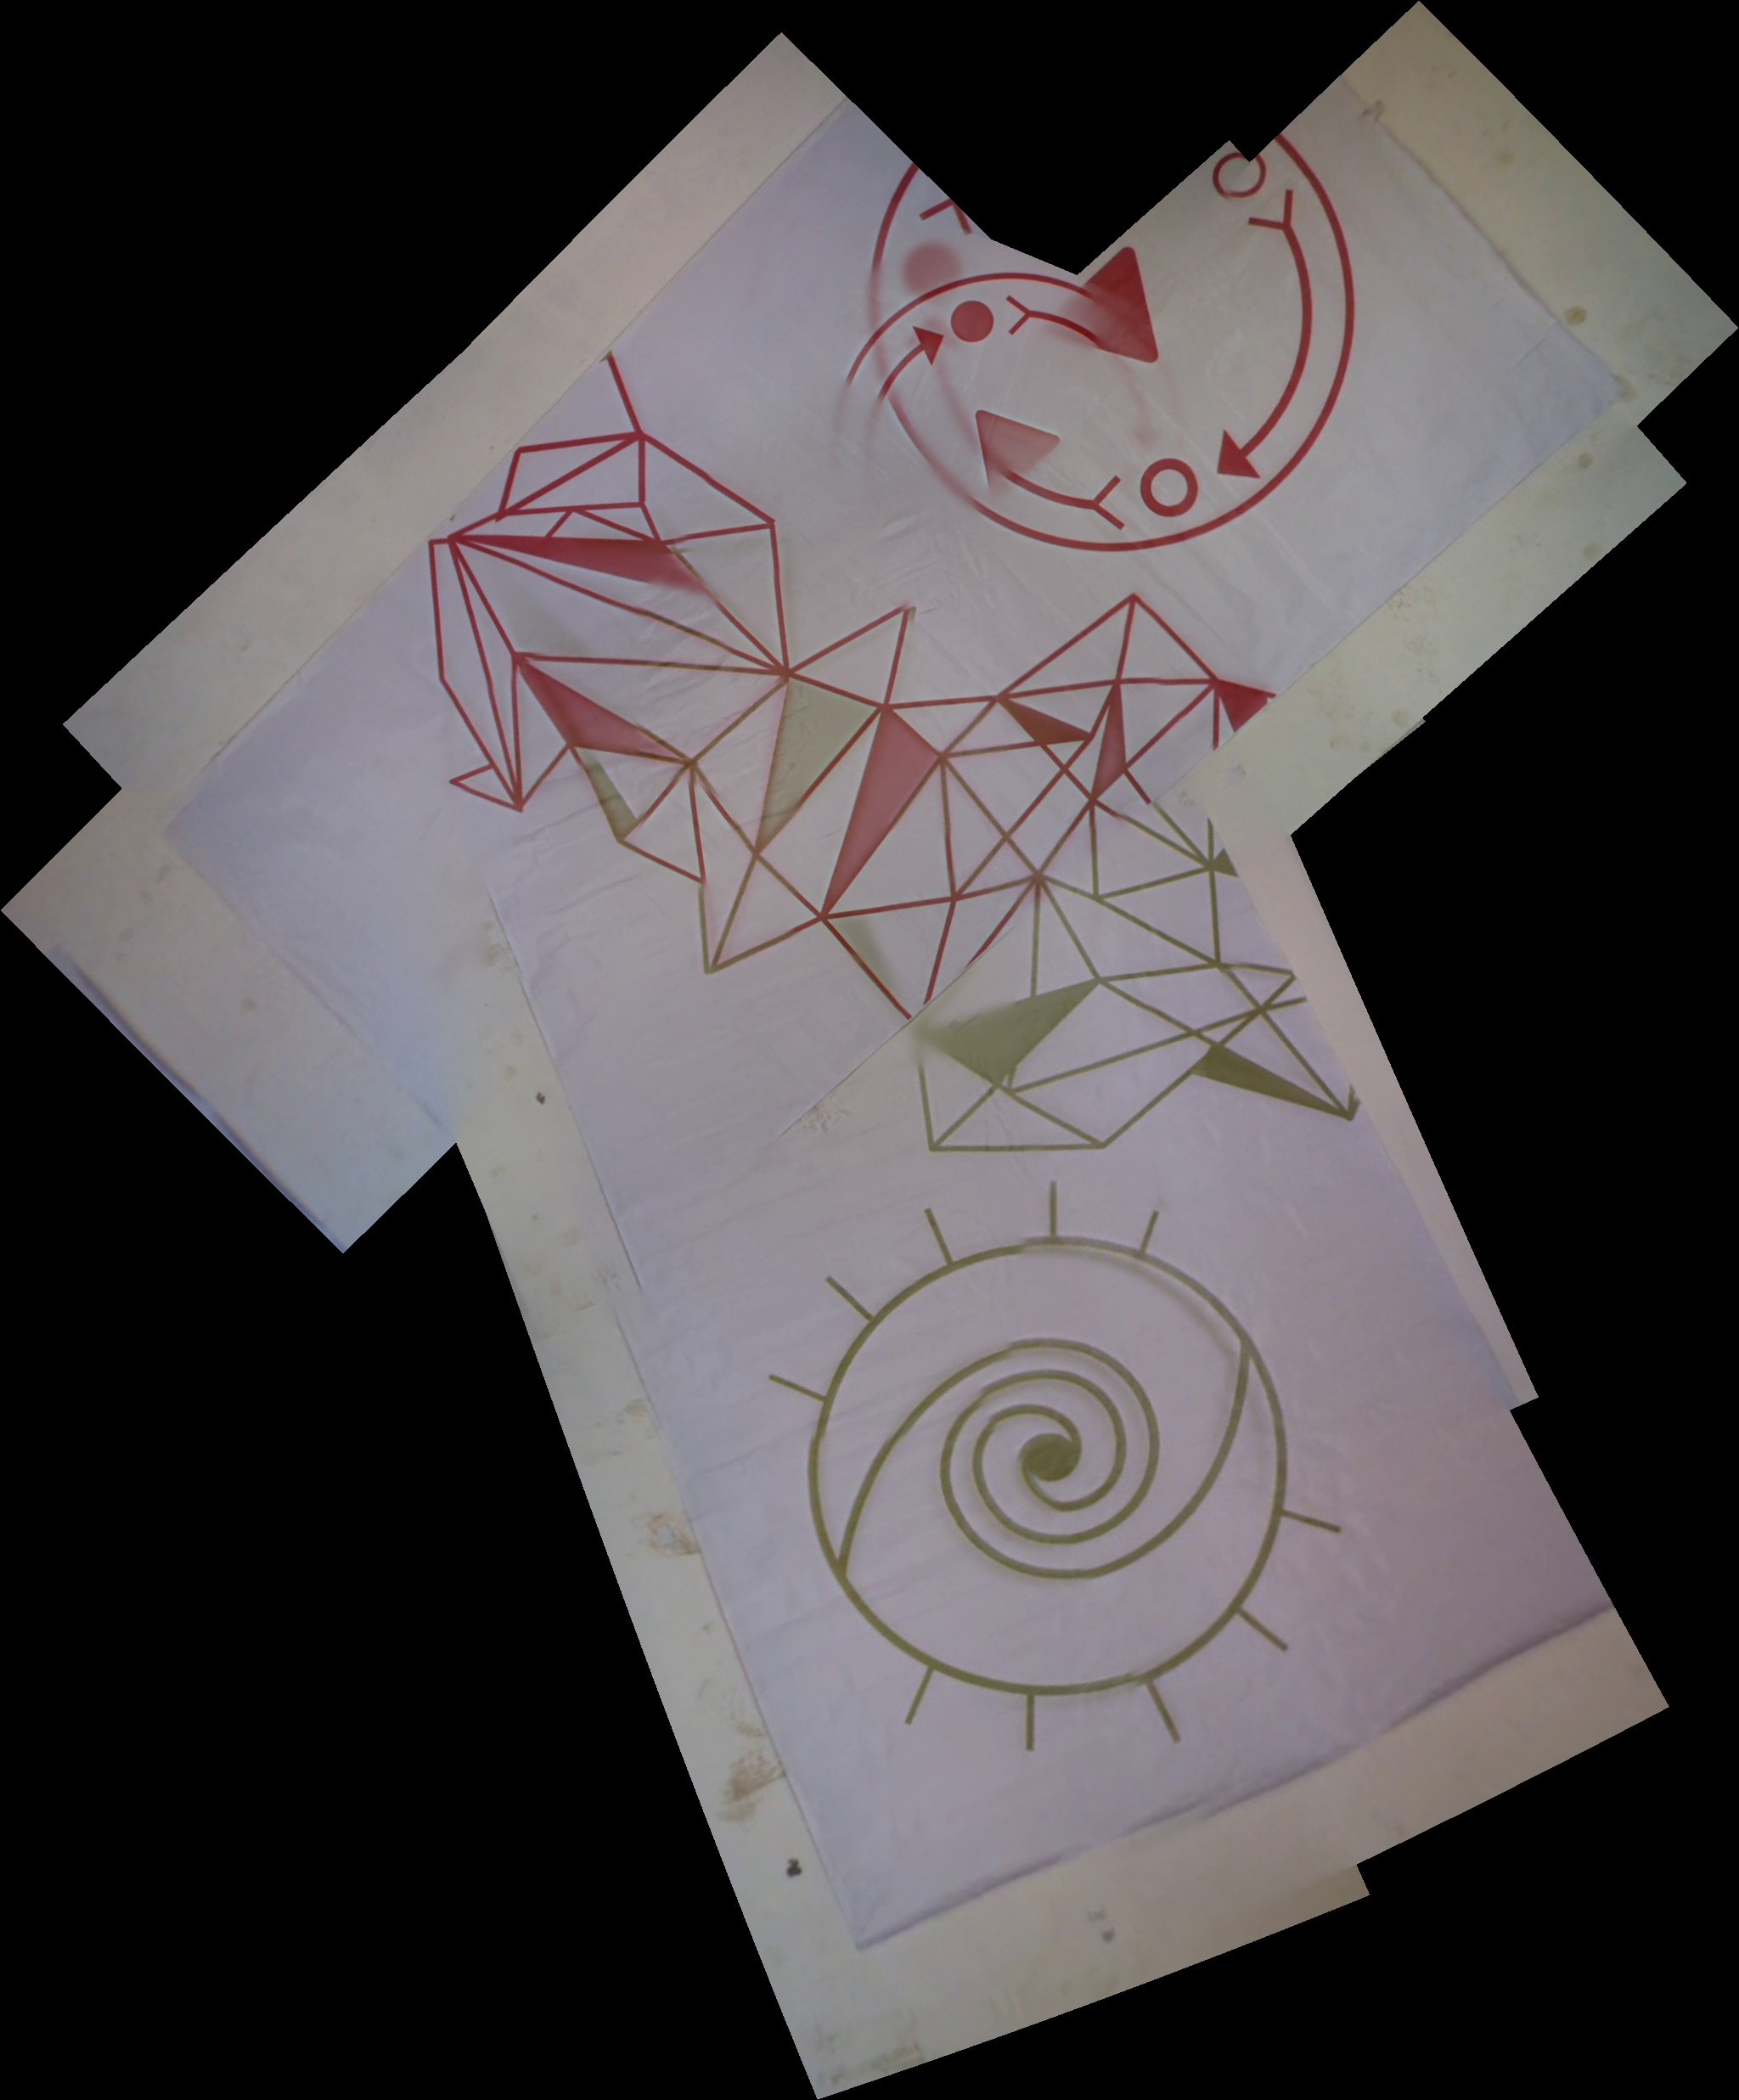
\includegraphics[width=\linewidth]{figures/green_red/autostich.jpg}
\caption{Autostitch Result}
\end{subfigure}
\begin{subfigure}[b]{0.3\textwidth}
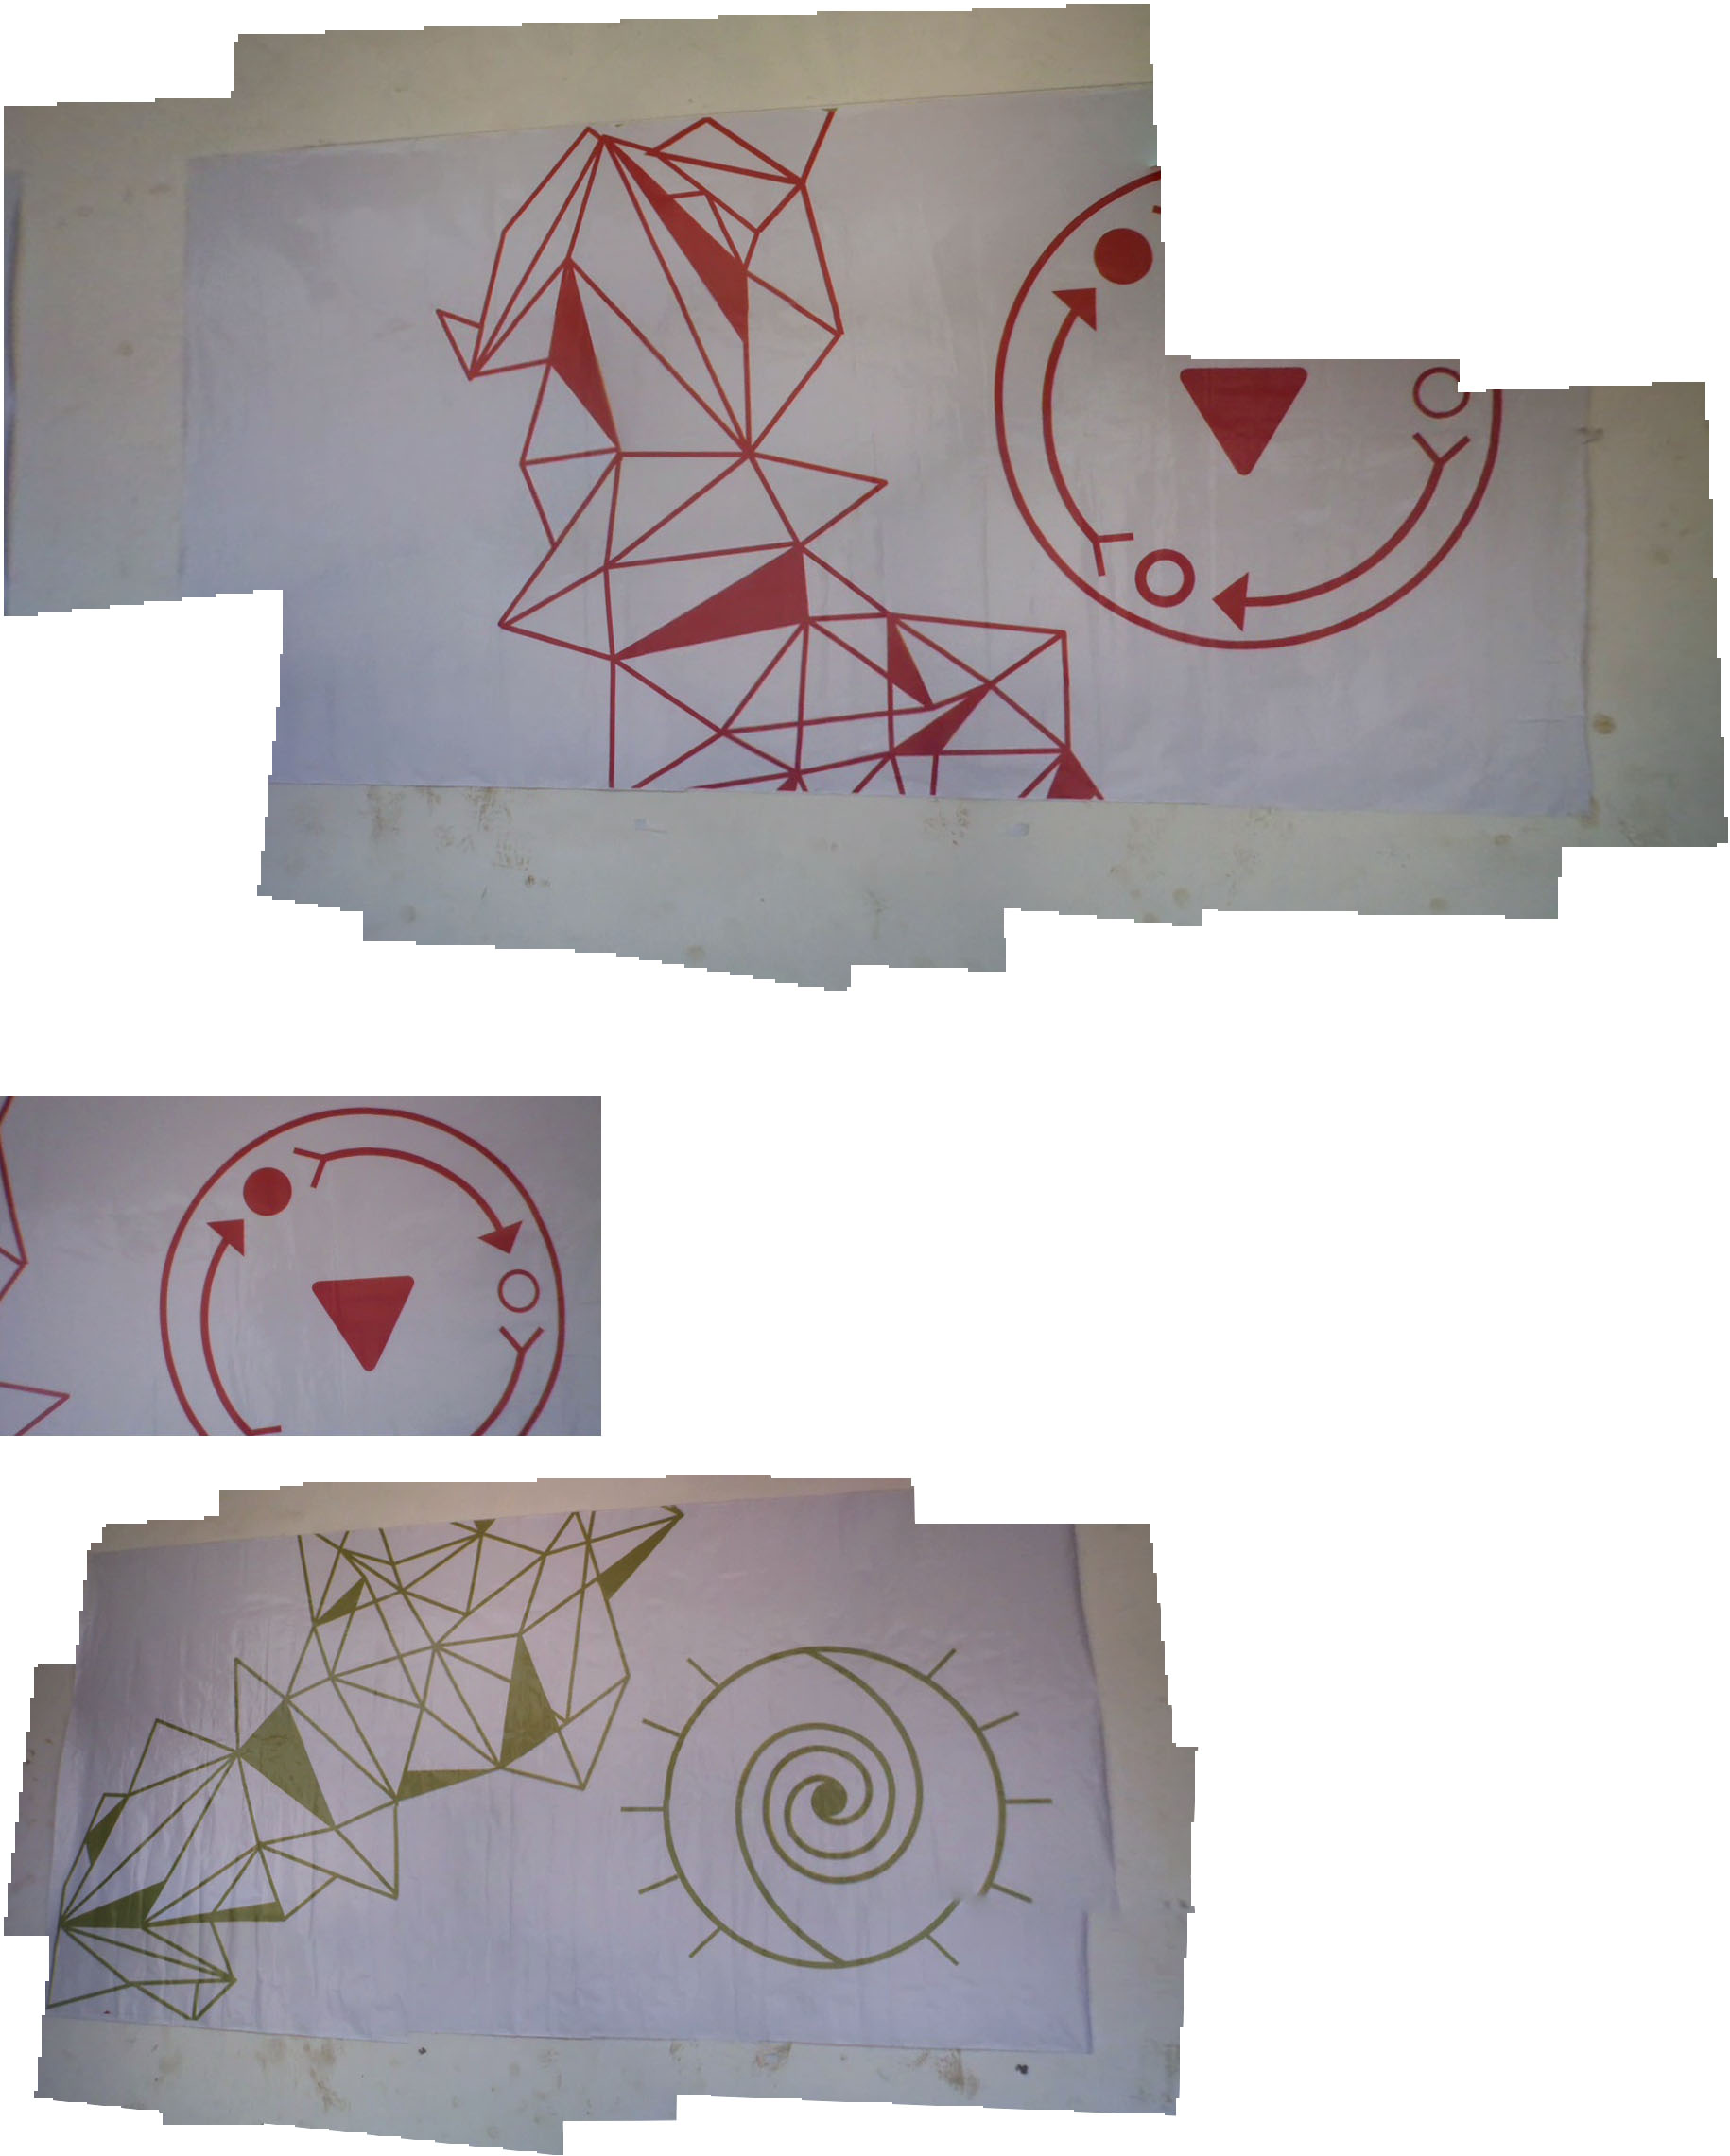
\includegraphics[width=\linewidth]{figures/green_red/photoshop_output.jpg}
\caption{Photoshop Result}
\end{subfigure}
\begin{subfigure}[b]{0.3\textwidth}
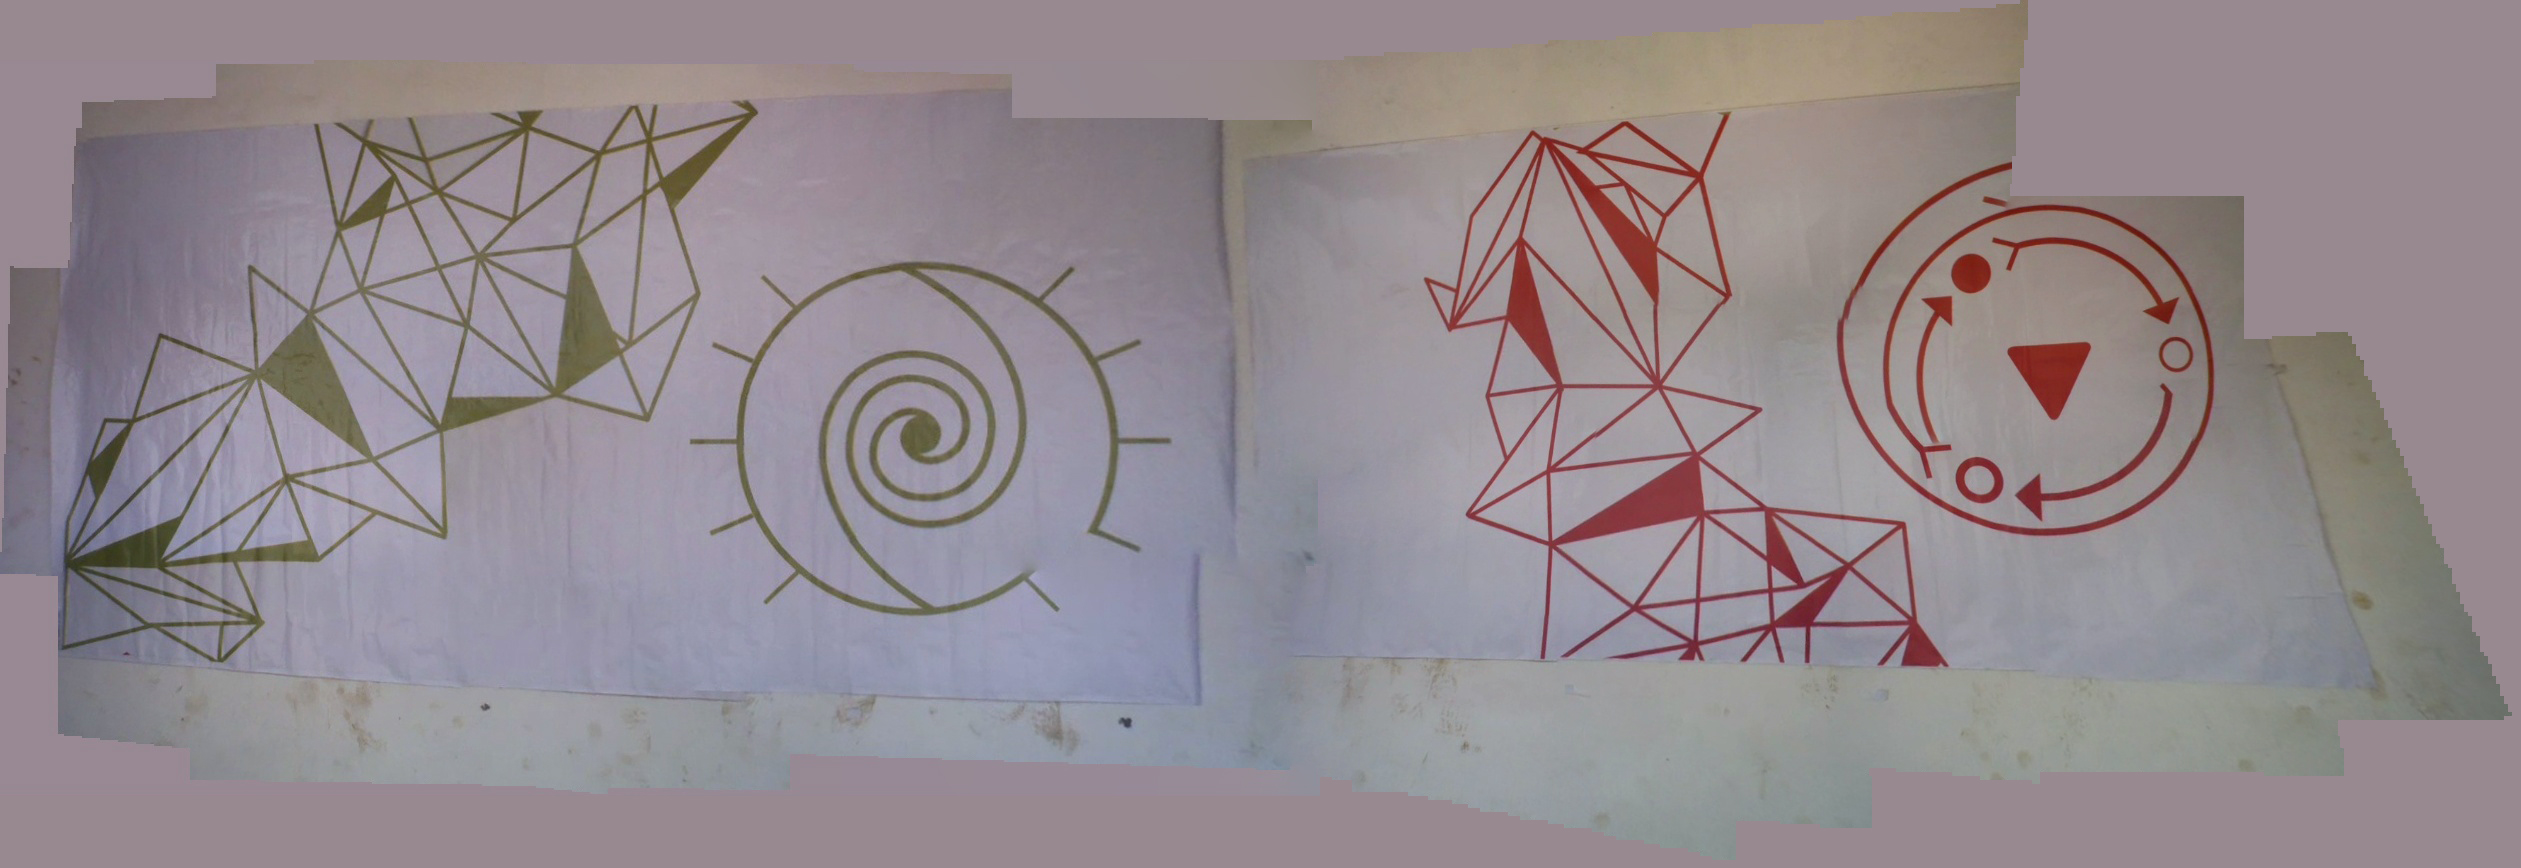
\includegraphics[width=\linewidth]{figures/green_red/our_result.jpg}
\caption{Our Result}
\end{subfigure}
\caption{Comparison of outputs of Autostich, Photoshop and our stitching
algorithm on the images selected of outdoor scene by our algorithm. Only our
output is able to shows individual panoramas at their respective location
approximately}
\label{fig:green_red_comparison}
\end{figure*}

Figure \ref{fig:green_red_comparison} shows the comparison of outputs of
state of the art stitchers with output of our algorithm.